\documentclass{beamer}
\usetheme{Madrid}
\usecolortheme{beaver}

\usepackage[utf8]{inputenc}
\usepackage{amsmath}
\usepackage{tikz}
\usetikzlibrary{arrows.meta, positioning}

\tikzset{
    bnode/.style={circle, draw, fill=black, text=white, minimum size=6mm, font=\footnotesize\bfseries},
    rnode/.style={circle, draw, fill=red!80!black, text=white, minimum size=6mm, font=\footnotesize\bfseries},
    nilnode/.style={rectangle, draw, fill=black, text=white, minimum size=3mm, font=\tiny},
    edge from parent/.style={draw, -Latex},
}

\title{Red-Black Trees: Insertion and Rebalancing}
\subtitle{BLG 202E -- Data Structures}
\author{Deniz Sipahi -- 150230006}
\date{May 11, 2026}
\institute{Istanbul Technical University}

\begin{document}

% Slide 1 -- Title
\begin{frame}
\titlepage
\end{frame}

% Slide 2 -- Motivation
\begin{frame}{1. Motivation -- Why Balance Matters}
\begin{itemize}
    \item A \textbf{Binary Search Tree (BST)} supports search, insert, and delete in $O(h)$ time, where $h$ is the tree height.
    \item In the \textbf{worst case}, a BST degenerates into a linked list: $h = n$, so operations become $O(n)$.
    \item A \textbf{balanced BST} guarantees $h = O(\log n)$, making all operations efficient.
    \item \textbf{Red-Black Trees} are one of the most widely used self-balancing BSTs.
\end{itemize}

\begin{block}{Key Insight}
Balancing is not free --- it requires extra bookkeeping. Red-Black Trees achieve this through coloring constraints and rotations.
\end{block}
\end{frame}

% Slide 3 -- Red-Black Tree Properties (with intuitions)
\begin{frame}{2. Red-Black Tree Properties}
Every Red-Black Tree satisfies these five invariants:
\begin{enumerate}
    \item Every node is either \textcolor{red}{\textbf{RED}} or \textbf{BLACK}.\\
          \textit{This binary labeling is what gives us a simple mechanism to enforce balance.}
    \item The root is always \textbf{BLACK}.\\
          \textit{This anchors the tree --- no violation can ``escape'' past the root.}
    \item Every leaf (NIL/null) is \textbf{BLACK}.\\
          \textit{Treating NILs as black simplifies the counting in Property 5.}
    \item If a node is \textcolor{red}{\textbf{RED}}, both its children must be \textbf{BLACK}.\\
          \textit{This prevents long chains of RED nodes, bounding the longest path.}
    \item All paths from a node to its descendant leaves have the same \textbf{black-height}.\\
          \textit{This is the core balance invariant --- it guarantees $O(\log n)$ height.}
\end{enumerate}
\end{frame}

% Slide 4 -- Node Structure (TikZ box diagram)
\begin{frame}{3. Node Structure}
Each node in a Red-Black Tree stores:

\vspace{0.5em}
\begin{center}
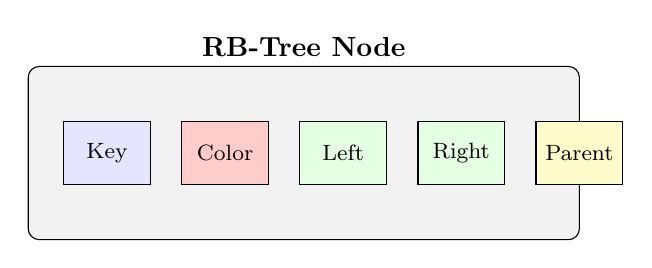
\begin{tikzpicture}
    \node[draw, rounded corners, minimum width=7cm, minimum height=2.2cm, fill=gray!10] (box) {};
    \node[above] at (box.north) {\textbf{RB-Tree Node}};
    \node[draw, fill=blue!10, minimum width=1.1cm, minimum height=0.8cm] at (-2.5,0) {\footnotesize Key};
    \node[draw, fill=red!20, minimum width=1.1cm, minimum height=0.8cm] at (-1.0,0) {\footnotesize Color};
    \node[draw, fill=green!10, minimum width=1.1cm, minimum height=0.8cm] at (0.5,0) {\footnotesize Left};
    \node[draw, fill=green!10, minimum width=1.1cm, minimum height=0.8cm] at (2.0,0) {\footnotesize Right};
    \node[draw, fill=yellow!20, minimum width=1.1cm, minimum height=0.8cm] at (3.5,0) {\footnotesize Parent};
\end{tikzpicture}
\end{center}

\vspace{0.5em}
\begin{itemize}
    \item \textbf{Key}: the stored value used for ordering
    \item \textbf{Color}: RED or BLACK --- used to maintain balance invariants
    \item \textbf{Left / Right}: pointers to child subtrees
    \item \textbf{Parent}: pointer to the parent (needed for fix-up traversal)
\end{itemize}
\end{frame}

% Slide 5 -- Insertion Base Steps
\begin{frame}{4. Insertion -- Base Steps}
Inserting into a Red-Black Tree follows two phases:

\begin{enumerate}
    \item \textbf{Standard BST Insert}: Insert the new node as a leaf, colored \textcolor{red}{\textbf{RED}}.
    \item \textbf{Fix-up Phase}: Restore any violated RB-tree properties.
\end{enumerate}

\vspace{0.5em}
Possible violations after inserting a RED node:
\begin{itemize}
    \item \textbf{Property 2}: The new node might be the root (root must be BLACK).
    \item \textbf{Property 4}: The new node's parent might also be RED (no two consecutive RED nodes).
\end{itemize}

\begin{block}{Why insert as RED?}
Inserting as RED preserves Property 5 (black-height) automatically. We only risk violating Property 4, which is easier to fix locally.
\end{block}
\end{frame}

% Slide 6 -- Fix-up Cases 1 & 2 (with TikZ)
\begin{frame}{5. Fix-up Cases 1 \& 2}
\textbf{Case 1 -- Uncle is RED (Recoloring):}
\begin{itemize}
    \item Recolor parent and uncle to BLACK, grandparent to RED.
    \item Move the pointer up to grandparent and repeat fix-up.
\end{itemize}

\vspace{0.3em}
\textbf{Case 2 -- Uncle is BLACK, zig-zag (Rotation):}
\begin{itemize}
    \item The new node is on the \emph{opposite side} of its parent relative to grandparent.
    \item Perform a rotation on the parent to straighten the path $\rightarrow$ becomes Case 3.
\end{itemize}

\vspace{0.3em}
\begin{center}
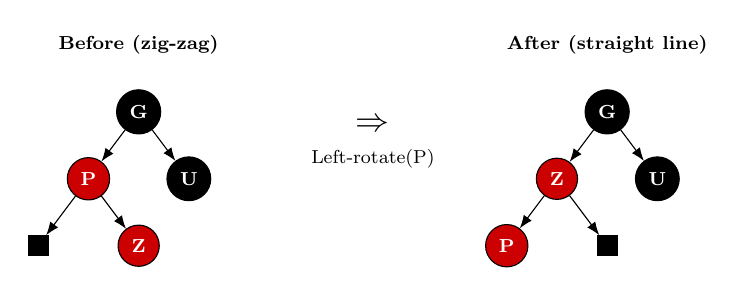
\begin{tikzpicture}[level distance=10mm, sibling distance=15mm, scale=0.85, transform shape]
    % Before rotation
    \node at (-2.5, 1.5) {\footnotesize \textbf{Before (zig-zag)}};
    \node[bnode] (g1) at (-2.5, 0.5) {G}
        child { node[rnode] (p1) {P}
            child { node[nilnode] {} }
            child { node[rnode] (z1) {Z} }
        }
        child { node[bnode] (u1) {U} };

    % Arrow
    \node at (1.0, 0.3) {\Large $\Rightarrow$};
    \node at (1.0, -0.2) {\footnotesize Left-rotate(P)};

    % After rotation
    \node at (4.5, 1.5) {\footnotesize \textbf{After (straight line)}};
    \node[bnode] (g2) at (4.5, 0.5) {G}
        child { node[rnode] (z2) {Z}
            child { node[rnode] (p2) {P} }
            child { node[nilnode] {} }
        }
        child { node[bnode] (u2) {U} };
\end{tikzpicture}
\end{center}
\end{frame}

% Slide 7 -- Fix-up Case 3 + Example
\begin{frame}{6. Fix-up Case 3 + Worked Example}
\textbf{Case 3 -- Uncle is BLACK, straight line (Rotate + Recolor):}
\begin{itemize}
    \item Rotate on the grandparent in the opposite direction.
    \item Swap colors of parent and grandparent.
\end{itemize}

\vspace{0.3em}
\textbf{Example:} Insert $15$ into the tree $\{10_B, 5_B, 20_R, 17_B\}$:
\begin{center}
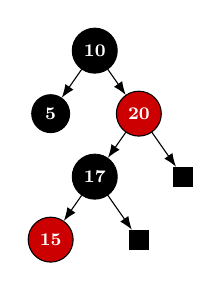
\begin{tikzpicture}[level distance=10mm, sibling distance=14mm, scale=0.8, transform shape]
    \node[bnode] {10}
        child { node[bnode] {5} }
        child { node[rnode] {20}
            child { node[bnode] {17}
                child { node[rnode] {15} }
                child { node[nilnode] {} }
            }
            child { node[nilnode] {} }
        };
\end{tikzpicture}
\end{center}
\footnotesize Node $15$ (RED) inserted under $17$ (BLACK). Parent is BLACK $\Rightarrow$ no violation occurs in this sub-case. (A violation would occur if $17$ were RED.)
\end{frame}

% Slide 8 -- Summary
\begin{frame}{7. Summary \& Key Takeaways}
\begin{itemize}
    \item Red-Black Trees maintain balance through \textbf{3 fix-up cases} after insertion:
    \begin{enumerate}
        \item \textbf{Recolor} (uncle is RED)
        \item \textbf{Rotate to straighten} (zig-zag, uncle is BLACK)
        \item \textbf{Rotate + recolor} (straight line, uncle is BLACK)
    \end{enumerate}
    \item The fix-up process involves \textbf{recoloring} and at most \textbf{2 rotations}.
    \item All operations (insert, delete, search) run in $O(\log n)$ time.
\end{itemize}

\begin{block}{Remember}
Think of the Red-Black Tree as a traffic system: RED means ``stop and check above,'' BLACK means ``all clear.'' Violations propagate upward like escalating a complaint to management.
\end{block}

\footnotesize{Reference: Cormen et al., \textit{Introduction to Algorithms}, 4th Ed., Chapter 13.}
\end{frame}

\end{document}
